\documentclass[tikz, border=5pt]{standalone}

\begin{document}
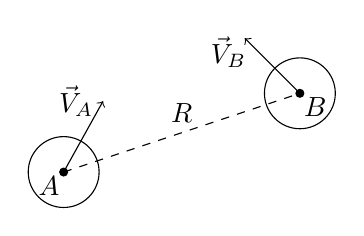
\begin{tikzpicture}

    %% Collision diagram

    % Mass A
    \coordinate (A) at (0,0);
    \draw[fill] (A) circle (0.05) node[below left=-2] {\( A \)};
    \draw (A) circle (0.45);
    \draw[->] (A) -- ++(0.5,0.9) node[left] {\( \vec{V}_A \)};

    % Mass B
    \coordinate (B) at (3,1);
    \draw[fill] (B) circle (0.05) node[below right=-2] {\( B \)};
    \draw (B) circle (0.45);
    \draw[->] (B) -- ++(-0.7,0.7) node[below left=-4] {\( \vec{V}_B \)};

    % Line of separation
    \draw[dashed] (A) -- (B) node[midway, above] {\( R \)};

\end{tikzpicture}
\end{document}
